\part{Hệ hỗ trợ quyết định}
\label{part:ch4}
% Long code identifiers cannot be hyphenated, so this chapter allows looser inter-word spacing.
\begingroup
\sloppy

Chương này trình bày thành phần hỗ trợ quyết định (\textit{Decision Support System}, DSS) xây trên kho dữ liệu. DSS xếp mỗi hồ sơ vào một thang hạng A--E, gắn một chính sách cho hạng đó và giải thích lý do. Trưởng phòng rủi ro dùng DSS để thử chính sách khác trên cả danh mục trước khi áp dụng.

%======================================================================
\section{Bài toán quyết định và vai trò của DSS}
\label{sec:dss-problem}

Thẩm định tín dụng là một quyết định bán cấu trúc (mục~\ref{sec:semi-structured}), nên DSS chỉ đề xuất, không tự động quyết định.

\medskip

Kho dữ liệu là nền của DSS. Mô hình học từ \texttt{mart.v\_application\_wide} trong kho, không đọc tập tin gốc. Tỷ lệ vỡ nợ của phân khúc và của luật tính bằng SQL trên kho. Kết quả chấm điểm ghi ngược vào kho thành hai bảng sự kiện, nên bảng điều khiển (\textit{dashboard}) và DSS luôn thấy cùng một dữ liệu.

\medskip

Bảng~\ref{tab:simon-phases} (Chương~\ref{part:ch1}) gắn bốn giai đoạn của Simon với các thành phần hệ thống. Trên web, giai đoạn Nhận thức dùng các trang \textbf{Overview}, \textbf{Analytics} và \textbf{Explorer}; Thiết kế dùng \textbf{Playground}; Lựa chọn dùng \textbf{Application details}.

%======================================================================
\section{Thang A--E và luồng DSS}
\label{sec:dss-flow}

Hệ thống dùng một thang hạng A--E duy nhất. Hạng được xác định theo tỷ lệ rủi ro, tức PD của hồ sơ (hạng điểm) hoặc tỷ lệ vỡ nợ lịch sử của nhóm vi phạm luật (hạng luật). Bảng~\ref{tab:grade-scale} cho các ngưỡng $1\%$, $7\%$, $13\%$ và $20\%$. Mỗi khoảng tính cận dưới, không tính cận trên; tỷ lệ đúng $7\%$ thuộc hạng C.

\begin{table}[H]
	\centering
	\caption{Thang hạng A--E}
	\label{tab:grade-scale}
	\footnotesize
	\begin{tabular}{c l l l}
		\toprule
		\textbf{Hạng} & \textbf{Tỷ lệ rủi ro} & \textbf{Ý nghĩa} & \textbf{Nhãn trên web}  \\
		\midrule
		A             & dưới $1\%$            & Rất tin tưởng    & \textbf{Very low risk}  \\
		B             & $1\%$--$7\%$          & Tin tưởng        & \textbf{Low risk}       \\
		C             & $7\%$--$13\%$         & Rủi ro vừa phải  & \textbf{Moderate risk}  \\
		D             & $13\%$--$20\%$        & Rủi ro cao       & \textbf{High risk}      \\
		E             & từ $20\%$             & Rủi ro rất cao   & \textbf{Very high risk} \\
		\bottomrule
	\end{tabular}
\end{table}

Thang này dùng cho ba loại hạng:
\begin{itemize}[topsep=0pt, itemsep=1pt]
	\item \textbf{Hạng điểm:} Xác suất vỡ nợ (\textit{probability of default}, PD) do mô hình ước lượng cho riêng hồ sơ, quy về thang A--E.
	\item \textbf{Hạng luật:} Hạng xấu nhất trong các luật mà hồ sơ vi phạm; hồ sơ không vi phạm luật nào thì không có hạng luật.
	\item \textbf{Hạng cuối:} Hạng xấu hơn trong hai hạng trên, và là căn cứ chọn chính sách.
\end{itemize}

Với thứ tự A $<$ B $<$ C $<$ D $<$ E theo mức rủi ro, hạng cuối là
\begin{equation}
	g_{\text{cuối}} = \max\left(g_{\text{điểm}},\ g_{\text{luật}}\right),
\end{equation}
và bằng $g_{\text{điểm}}$ khi hồ sơ không vi phạm luật nào. Luật chỉ hạ hạng, không bao giờ nâng hạng. Hạng A vì vậy chỉ đạt được khi điểm cá nhân rất tốt và hồ sơ không vi phạm luật nào.

\medskip

Hình~\ref{fig:dss_flow} tóm tắt luồng xử lý một hồ sơ. Phần chuẩn bị chạy mỗi lần ETL, phần chấm điểm chạy bằng lệnh \texttt{hcdw score} hoặc qua API.

\begin{figure}[H]
	\centering
	\mermaidfile[width=\linewidth, keepaspectratio]{diagrams/dss_flow.mmd}
	\caption{Luồng hệ hỗ trợ quyết định}
	\label{fig:dss_flow}
\end{figure}

%======================================================================
\section{Mô hình PD và hạng điểm}
\label{sec:dss-model}
Mô hình dùng $26$ đặc trưng lấy từ \texttt{mart.v\_application\_wide}: $18$ đặc trưng số và $8$ đặc trưng phân loại. Nhóm đặc trưng gồm điểm tín dụng ngoài, số tiền vay và thu nhập, các tỷ lệ suy ra, tuổi và thâm niên, lịch sử tại trung tâm tín dụng (\textit{Credit Bureau}), hồ sơ vay trước đây tại Home Credit và lịch sử trả góp. Giới tính (\texttt{gender}) không thuộc mô hình; nó chỉ là một chiều phân tích.

\medskip

Mô hình là LightGBM với kiểm định chéo phân tầng $5$ phần (\textit{stratified 5-fold cross-validation}). Mỗi khoản vay lịch sử nhận một PD dự đoán ngoài phần (\textit{out-of-fold}, OOF) từ mô hình chưa từng thấy nó. Nhờ vậy, tỷ lệ vỡ nợ theo hạng trên khoản vay lịch sử không bị thổi phồng do rò rỉ nhãn. Hồ sơ mới được chấm bằng mô hình huấn luyện trên toàn bộ khoản vay lịch sử.

\medskip

Ngưỡng hạng là xác suất thật, nên PD phải khớp với tỷ lệ vỡ nợ thực tế. Mô hình không dùng trọng số lớp. Xác suất thô được hiệu chỉnh bằng hồi quy đơn điệu (\textit{isotonic regression}) khớp trên PD OOF. Kết quả trong \texttt{models/metrics.json}, trên $307.511$ khoản vay lịch sử:
\begin{itemize}[topsep=0pt, itemsep=1pt]
	\item \textbf{Độ phân biệt:} Diện tích dưới đường cong ROC (\textit{AUC}) của PD OOF đã hiệu chỉnh là $0{,}7586$; trước hiệu chỉnh là $0{,}7581$.
	\item \textbf{Độ chính xác xác suất:} Điểm Brier (\textit{Brier score}) là $0{,}0678$.
	\item \textbf{Mức trung bình:} PD trung bình OOF là $8{,}07\%$, bằng tỷ lệ vỡ nợ chung.
	\item \textbf{Hiệu chỉnh:} Ở $10$ nhóm thập phân vị PD, PD trung bình và tỷ lệ vỡ nợ thực tế gần như trùng nhau, từ $1{,}11\%$ so với $1{,}10\%$ ở nhóm thấp nhất tới $27{,}15\%$ so với $27{,}17\%$ ở nhóm cao nhất.
\end{itemize}

Bộ hiệu chỉnh được khớp và được đo trên cùng một tập PD OOF. Vì vậy điểm Brier và bảng hiệu chỉnh cho thấy độ khớp, chưa phải kết quả kiểm định; mục~\ref{sec:eval-limits} nêu giới hạn này.

\medskip

Bảng~\ref{tab:shap-top} liệt kê năm đặc trưng có trung bình $|\text{SHAP}|$ lớn nhất trên khoản vay lịch sử. Điểm tín dụng ngoài ảnh hưởng lớn nhất, gấp khoảng bốn lần đặc trưng thứ hai.

\begin{table}[H]
	\centering
	\caption{Năm đặc trưng ảnh hưởng lớn nhất tới PD}
	\label{tab:shap-top}
	\footnotesize
	\begin{tabular}{c l l r}
		\toprule
		\textbf{\#} & \textbf{Đặc trưng}            & \textbf{Nhãn trên web}                  & \textbf{Trung bình $|\text{SHAP}|$} \\
		\midrule
		1           & \texttt{ext\_source\_mean}    & \textbf{Average external credit score}  & $0{,}548$                           \\
		2           & \texttt{credit\_to\_goods}    & \textbf{Credit to goods price ratio}    & $0{,}135$                           \\
		3           & \texttt{years\_employed}      & \textbf{Years employed}                 & $0{,}134$                           \\
		4           & \texttt{late\_payment\_ratio} & \textbf{Share of instalments paid late} & $0{,}133$                           \\
		5           & \texttt{education\_type}      & \textbf{Education}                      & $0{,}105$                           \\
		\bottomrule
	\end{tabular}
\end{table}

\section{Luật và hạng luật}
\label{sec:dss-rules}

Luật là một điều kiện có mã, được kiểm tra trên một hồ sơ. Hồ sơ thỏa điều kiện thì vi phạm luật. Tỷ lệ rủi ro của luật là tỷ lệ vỡ nợ của các khoản vay lịch sử vi phạm luật đó. Tỷ lệ này được quy về hạng theo đúng thang A--E của hạng điểm.

\medskip

Mô hình chấm từng cá nhân, nhưng chuyên viên khó kiểm tra lại cách mô hình chấm. Luật có mã, điều kiện và tỷ lệ rõ ràng, nên chuyên viên đọc và kiểm tra được. Luật chỉ hạ hạng vì không phân khúc nào có tỷ lệ vỡ nợ dưới $1\%$; thấp nhất là $2{,}99\%$, hạng B. Nếu hạng phân khúc luôn được gộp vào hạng cuối, không hồ sơ nào đạt hạng A.

\subsection{Luật phân khúc BR-SEG-01}
\label{sec:dss-segment-rule}
Phân khúc là tổ hợp giá trị của bốn thuộc tính ổn định, dễ giải thích:
\begin{itemize}[topsep=0pt, itemsep=1pt]
	\item \textbf{Lịch sử tín dụng} (\texttt{credit\_history\_status}): \mintinline[fontsize=\small]{sql}|'No bureau'| (không có dữ liệu Credit Bureau), \mintinline[fontsize=\small]{sql}|'Clean history'| (có lịch sử, không đang quá hạn) hoặc \mintinline[fontsize=\small]{sql}|'Current overdue'| (đang quá hạn).
	\item \textbf{Nhóm tuổi} (\texttt{age\_band}): Năm nhóm $18$--$24$, $25$--$34$, $35$--$44$, $45$--$54$ và từ $55$ tuổi.
	\item \textbf{Nhóm thu nhập} (\texttt{income\_group}): Bốn loại thu nhập lớn là \mintinline[fontsize=\small]{sql}|'Working'|, \mintinline[fontsize=\small]{sql}|'Commercial associate'|, \mintinline[fontsize=\small]{sql}|'Pensioner'| và \mintinline[fontsize=\small]{sql}|'State servant'|. Các loại khác gộp thành \mintinline[fontsize=\small]{sql}|'Other'|.
	\item \textbf{Hạng vùng} (\texttt{region\_rating\_client}): $1$, $2$ hoặc $3$.
\end{itemize}

Tổng cộng có $3 \times 5 \times 5 \times 3 = 225$ phân khúc. Khung nhìn \texttt{mart.segment\_risk} có một dòng cho mỗi phân khúc, kể cả phân khúc chưa có khoản vay lịch sử nào. Vì vậy hồ sơ mới luôn tra được phân khúc.

\medskip

Phân khúc dưới $500$ khoản vay lịch sử có tỷ lệ không đáng tin. Khi đó hệ thống lùi về cấp cha (\textit{fallback}) theo thứ tự trong Bảng~\ref{tab:segment-fallback}, và dùng cấp đầu tiên có từ $500$ khoản vay trở lên. Lịch sử tín dụng được giữ tới cuối vì gắn trực tiếp với hành vi trả nợ.

\begin{table}[H]
	\centering
	\caption{Cấp lấy tỷ lệ của luật phân khúc}
	\label{tab:segment-fallback}
	\footnotesize
	\begin{tabular}{c p{0.42\textwidth} r r}
		\toprule
		\textbf{Cấp} & \textbf{Nhóm dùng để tính tỷ lệ}    & \textbf{Số phân khúc} & \textbf{Khoản vay lịch sử} \\
		\midrule
		4            & Đủ bốn thuộc tính (chính phân khúc) & $61$                  & $293.304$                  \\
		3            & Bỏ hạng vùng                        & $47$                  & $11.596$                   \\
		2            & Bỏ thêm nhóm thu nhập               & $102$                 & $2.506$                    \\
		1            & Chỉ còn lịch sử tín dụng            & $15$                  & $105$                      \\
		0            & Toàn bộ khoản vay lịch sử           & $0$                   & $0$                        \\
		\midrule
		             & \textbf{Tổng}                       & $225$                 & $307.511$                  \\
		\bottomrule
	\end{tabular}
\end{table}

Mỗi phân khúc đều có một hạng, nên cần quy định hạng nào mới bị coi là vi phạm. Tập kích hoạt là \{D, E\}. Với tập này, luật gắn cờ $20.320$ khoản vay lịch sử ($6{,}61\%$, tỷ lệ vỡ nợ chung $15{,}12\%$) và $3.031$ hồ sơ mới ($6{,}22\%$). Tập \{E\} chỉ gắn cờ $0{,}71\%$ khoản vay lịch sử, gần như không có tác dụng. Tập \{C, D, E\} gắn cờ $62{,}3\%$ và lấn át hạng điểm.

Cả nhóm luật phân khúc dùng một mã \texttt{BR-SEG-01}. Mỗi lần vi phạm lưu khóa phân khúc (\texttt{segment\_key}) và nhóm thực sự cung cấp tỷ lệ (\texttt{rate\_key}); thuộc tính đã bỏ khi lùi cấp ghi là \texttt{*}. Tỷ lệ và hạng của lần vi phạm là tỷ lệ và hạng của chính phân khúc đó.

\subsection{Luật nghiệp vụ BR-RF-01..05}
\label{sec:dss-business-rules}

Luật nghiệp vụ dựa trên hành vi tín dụng trong quá khứ. Mỗi luật là một biểu thức SQL trên các cột của bảng tổng hợp hồ sơ trong kho, khai báo trong tập tin cấu hình \texttt{configs/settings.yaml}. Khi chấm hàng loạt, biểu thức được bọc như sau, nên giá trị thiếu nghĩa là không vi phạm:
\begin{center}
	\mintinline[fontsize=\small]{sql}|COALESCE((sql), FALSE)|
\end{center}

Bảng~\ref{tab:business-rules} liệt kê sáu luật. Số vi phạm và tỷ lệ vỡ nợ tính trên khoản vay lịch sử. Cột cuối đếm trên mọi hồ sơ (đã chấm), giống cột \textbf{Loans hit} trên trang \textbf{Playground}.

\begin{table}[H]
	\centering
	\caption{Danh mục luật và thống kê vi phạm}
	\label{tab:business-rules}
	\footnotesize
	\begin{tabular}{l p{0.3\textwidth} r r c r}
		\toprule
		\textbf{Mã} & \textbf{Điều kiện}                                                 & \makecell[r]{\textbf{Vi phạm}\\\textbf{(lịch sử)}} & \makecell[r]{\textbf{Tỷ lệ}\\\textbf{vỡ nợ}} & \textbf{Hạng} & \makecell[r]{\textbf{Vi phạm}\\\textbf{(mọi hồ sơ)}} \\
		\midrule
		BR-SEG-01   & Hạng phân khúc thuộc \{D, E\}                                      & $20.320$                                           & $15{,}12\%$                                  & D             & $23.351$                                             \\
		BR-RF-01    & \mintinline[fontsize=\footnotesize]{sql}|prev_approval_rate < 0.5| & $19.056$                                           & $15{,}10\%$                                  & D             & $22.406$                                             \\
		BR-RF-02    & \mintinline[fontsize=\footnotesize]{sql}|late_payment_ratio > 0.2| & $37.462$                                           & $11{,}99\%$                                  & C             & $42.419$                                             \\
		BR-RF-03    & \mintinline[fontsize=\footnotesize]{sql}|max_dpd_days > 90|        & $12.132$                                           & $9{,}83\%$                                   & C             & $14.417$                                             \\
		BR-RF-04    & \mintinline[fontsize=\footnotesize]{sql}|has_current_overdue|      & $3.345$                                            & $16{,}11\%$                                  & D             & $3.812$                                              \\
		BR-RF-05    & \mintinline[fontsize=\footnotesize]{sql}|late_payment_ratio > 0.5| & $2.244$                                            & $16{,}44\%$                                  & D             & $2.469$                                              \\
		\bottomrule
	\end{tabular}
\end{table}

Dòng BR-SEG-01 trong bảng chỉ để tham khảo. Mỗi lần vi phạm luật phân khúc dùng tỷ lệ và hạng của chính phân khúc, nên có thể là D hoặc E. Một số điểm về các luật còn lại:
\begin{itemize}[topsep=0pt, itemsep=1pt]
	\item \textbf{BR-RF-03:} Tỷ lệ chỉ cao hơn mức chung $1{,}8$ điểm phần trăm, nhưng vẫn đạt hạng C nên hạ được hồ sơ A/B xuống C.
	\item \textbf{BR-RF-04:} $2.581$ trong $3.345$ khoản vay vi phạm đã bị luật phân khúc gắn cờ; $764$ khoản còn lại nằm trong phân khúc hạng C (nhóm $55+$), nên chỉ BR-RF-04 đưa chúng lên D.
	\item \textbf{BR-RF-05:} Là bậc nặng của BR-RF-02 và chuyển $1.851$ khoản vay từ hạng luật C lên D.
\end{itemize}

Một số luật ứng viên không được dùng. Luật theo tỷ lệ trả góp trên thu nhập (DTI) bị loại vì DTI gần như không phân biệt được rủi ro. Điều kiện \mintinline[fontsize=\small]{sql}|cnt_bureau_active >= 6| chỉ cao hơn ngưỡng D $0{,}38$ điểm phần trăm, nên hạng không ổn định. Không luật ứng viên nào cho hạng A hoặc B, nên hạng luật chỉ có thể là C, D hoặc E. Trên khoản vay lịch sử, $24{,}93\%$ có hạng luật (Bảng~\ref{tab:grade-distribution}).

%======================================================================
\section{Hạng cuối và chính sách theo hạng}
\label{sec:dss-policy}

Mỗi hạng cuối gắn đúng một chính sách: một quyết định và một hạn mức tối đa tính theo bội số thu nhập. Ba quyết định là Duyệt (\textbf{Approve}), Thẩm định thêm (\textbf{Manual review}) và Từ chối (\textbf{Reject}). Bảng~\ref{tab:policy-grade} cho chính sách hiện hành trong \texttt{configs/settings.yaml}.

\begin{table}[H]
	\centering
	\caption{Chính sách theo hạng cuối}
	\label{tab:policy-grade}
	\footnotesize
	\begin{tabular}{c l l r}
		\toprule
		\textbf{Hạng} & \textbf{Quyết định} & \textbf{Nhãn trên web} & \textbf{Hạn mức tối đa (lần thu nhập)} \\
		\midrule
		A             & Duyệt               & \textbf{Approve}       & $8{,}0$                                \\
		B             & Duyệt               & \textbf{Approve}       & $6{,}0$                                \\
		C             & Thẩm định thêm      & \textbf{Manual review} & $4{,}0$                                \\
		D             & Thẩm định thêm      & \textbf{Manual review} & $3{,}0$                                \\
		E             & Từ chối             & \textbf{Reject}        & $0$                                    \\
		\bottomrule
	\end{tabular}
\end{table}

Với hạng $g$ có hạn mức $k_g$, số tiền vay yêu cầu $C$ và thu nhập $I$, hạn mức khuyến nghị là
\begin{equation}
	H = C \times \min\left(1,\ \frac{k_g}{C / \min(I,\ 900.000)}\right) = \min\bigl(C,\ k_g \cdot \min(I,\ 900.000)\bigr).
\end{equation}
Trong kho, $C / \min(I, 900.000)$ là cột \texttt{credit\_to\_income}, và $H$ là cột \texttt{recommended\_credit}. Ngưỡng cắt thu nhập là $900.000$ (đơn vị tiền gốc); mọi số tiền trong chương giữ nguyên đơn vị của dữ liệu gốc. Ngưỡng này không viết cứng; hệ thống đọc nó từ kho lúc chạy. Hạng E có hạn mức $0$.

Tỷ lệ vỡ nợ theo tỷ lệ tiền vay trên thu nhập gần như phẳng, từ $7{,}04\%$ tới $8{,}85\%$ trên khoản vay lịch sử. Vì vậy hạn mức là công cụ giới hạn số tiền có thể mất, không phải công cụ phân loại rủi ro. Các mức $8{,}0$, $6{,}0$ và $4{,}0$ xấp xỉ phân vị $92$, $82$ và $62$ của tỷ lệ này trên khoản vay lịch sử. Hồ sơ hạng A hầu như không bị cắt hạn mức ($5{,}5\%$), còn hồ sơ hạng B bị cắt hạn mức khoảng $18{,}6\%$. Với C/D, hạn mức là mức tối đa nếu chuyên viên duyệt sau khi thẩm định thêm.

%======================================================================
\section{Giải thích đề xuất}
\label{sec:dss-explain}

Người đọc phần giải thích là chuyên viên thẩm định, không phải khách hàng. Phần giải thích đi theo đúng hai nguồn tạo ra hạng:
\begin{itemize}[topsep=0pt, itemsep=1pt]
	\item \textbf{Hạng điểm:} Giá trị SHAP (\textit{SHapley Additive exPlanations}) chia điểm rủi ro thành phần đóng góp của từng đặc trưng. Hệ thống hiển thị tối đa năm yếu tố làm tăng rủi ro và năm yếu tố làm giảm rủi ro, kèm tên nghiệp vụ, tên cột và giá trị của khách.
	\item \textbf{Hạng luật:} Danh sách mọi luật bị vi phạm, mỗi luật có mã, nhóm, tỷ lệ vỡ nợ của nhóm vi phạm và hạng.
	\item \textbf{Hạng cuối:} Một câu tóm tắt nêu nguồn quyết định hạng cuối và mức bị hạ hạng, ví dụ ``Downgraded from C to D by segment rule BR-SEG-01 and business rule BR-RF-04.''
\end{itemize}

SHAP được tính trên mô hình trước bước hiệu chỉnh, theo thang \textit{log-odds}. Hiệu chỉnh đơn điệu giữ nguyên thứ tự rủi ro, nên chiều tác động của từng yếu tố vẫn đúng với PD sau hiệu chỉnh. Giá trị SHAP chỉ dùng để so các yếu tố với nhau, không đọc thành điểm phần trăm PD.

\medskip

Ở cấp danh mục, hệ thống lấy trung bình $|\text{SHAP}|$ trên khoản vay lịch sử (Bảng~\ref{tab:shap-top}). Trưởng phòng rủi ro dùng phần này để kiểm tra logic của mô hình và xác nhận giới tính không ảnh hưởng tới kết quả.

%======================================================================
\section{Bảng của DSS trong kho dữ liệu}
\label{sec:dss-tables}

Kết quả của DSS nằm trong bốn bảng của kho, bên cạnh mô hình đa chiều ở Chương~\ref{part:ch2}. Bảng~\ref{tab:dss-tables} tóm tắt bốn bảng này.

\begin{table}[H]
	\centering
	\caption{Bảng DSS trong kho dữ liệu}
	\label{tab:dss-tables}
	\footnotesize
	\begin{tabular}{p{0.29\textwidth} p{0.19\textwidth} p{0.14\textwidth} p{0.28\textwidth}}
		\toprule
		\textbf{Bảng}                      & \textbf{Mức chi tiết}                 & \textbf{Nạp bởi}    & \textbf{Nội dung chính}                                                    \\
		\midrule
		\texttt{dw.dim\_risk\_grade}       & Một hạng ($5$ dòng)                   & ETL, từ cấu hình    & Khoảng tỷ lệ, nhãn, quyết định, hạn mức                                    \\
		\texttt{dw.dim\_rule}              & Một luật ($6$ dòng)                   & ETL, từ cấu hình    & Nhóm luật, nhãn, biểu thức SQL, cột cần                                    \\
		\texttt{dw.fact\_risk\_assessment} & Một hồ sơ đã chấm ($356.255$ dòng)    & \texttt{hcdw score} & PD, ba hạng, quyết định, hạn mức khuyến nghị, phân khúc và tỷ lệ phân khúc \\
		\texttt{dw.fact\_rule\_hit}        & Một lần vi phạm luật ($108.874$ dòng) & \texttt{hcdw score} & Mã luật, tỷ lệ, hạng; khóa phân khúc cho BR-SEG-01                         \\
		\bottomrule
	\end{tabular}
\end{table}

Bốn ràng buộc \mintinline[fontsize=\small]{sql}|CHECK| trên \texttt{fact\_risk\_assessment} giữ các bất biến của DSS ngay trong kho (mục~\ref{sec:star-schema}). Bảng sự kiện kết quả thẩm định lưu cả tỷ lệ phân khúc (\texttt{segment\_rate}) khi luật phân khúc không kích hoạt. Nhờ vậy mô phỏng chính sách xếp hạng lại phân khúc theo ngưỡng mới mà không chạy lại mô hình.

%======================================================================
\section{Kết quả trên dữ liệu thật}
\label{sec:dss-results}

Bảng~\ref{tab:grade-distribution} cho phân bố ba loại hạng trên khoản vay lịch sử. Mỗi ô ghi tỷ trọng và tỷ lệ vỡ nợ thực tế. Phân bố hạng cuối trên mọi hồ sơ (SM-1) nằm ở Bảng~\ref{tab:kpi-values}.

\begin{table}[H]
	\centering
	\caption{Phân bố hạng và tỷ lệ vỡ nợ theo hạng}
	\label{tab:grade-distribution}
	\footnotesize
	\begin{tabular}{l r r r}
		\toprule
		                   & \multicolumn{3}{c}{\textbf{Khoản vay lịch sử: tỷ trọng / tỷ lệ vỡ nợ}}                                                         \\
		\cmidrule(lr){2-4}
		\textbf{Hạng}      & \textbf{Hạng điểm}                                                     & \textbf{Hạng luật}        & \textbf{Hạng cuối}        \\
		\midrule
		A                  & $3{,}13\%$ / $0{,}64\%$                                                & --                        & $3{,}04\%$ / $0{,}62\%$   \\
		B                  & $58{,}86\%$ / $3{,}67\%$                                               & --                        & $49{,}02\%$ / $3{,}54\%$  \\
		C                  & $20{,}57\%$ / $9{,}79\%$                                               & $11{,}78\%$ / $9{,}98\%$  & $22{,}86\%$ / $8{,}29\%$  \\
		D                  & $9{,}21\%$ / $16{,}32\%$                                               & $12{,}44\%$ / $14{,}16\%$ & $16{,}40\%$ / $12{,}15\%$ \\
		E                  & $8{,}23\%$ / $28{,}85\%$                                               & $0{,}71\%$ / $22{,}21\%$  & $8{,}68\%$ / $28{,}02\%$  \\
		Không vi phạm luật & --                                                                     & $75{,}07\%$ / $6{,}63\%$  & --                        \\
		\bottomrule
	\end{tabular}
\end{table}

Tỷ lệ vỡ nợ tăng dần từ A tới E ở cả ba loại hạng, nên thang hạng đạt yêu cầu BR-07. Hạng A có xuất hiện ($3{,}13\%$ theo hạng điểm), nên kiểm tra áp dụng cho cả năm hạng. Hạng cuối D chỉ vỡ nợ $12{,}15\%$, thấp hơn ngưỡng $13\%$. Lý do là nhiều hồ sơ B/C bị luật hạ xuống D.

\medskip

Bảng~\ref{tab:kpi-values} (Chương~\ref{part:ch1}) ghi kết quả của chính sách hiện hành theo ba phạm vi. Hồ sơ vi phạm ít nhất một luật chiếm $24{,}93\%$ khoản vay lịch sử, $24{,}43\%$ hồ sơ mới và $24{,}86\%$ mọi hồ sơ. Nhóm được duyệt có tỷ lệ vỡ nợ $3{,}37\%$, so với $8{,}07\%$ của toàn bộ khoản vay lịch sử.

\medskip

Luật đọc lại một phần thông tin mà mô hình đã dùng, như trả trễ, quá hạn và lịch sử Credit Bureau. Vì vậy, khoản vay bị hạ hạng vẫn vỡ nợ ở mức gần hạng điểm ban đầu, không gần mức của hạng mà luật gán. Khoản vay hạng điểm B bị hạ xuống C vỡ nợ $4{,}08\%$, bị hạ xuống D vỡ nợ $4{,}61\%$. Trong khi đó khoản vay có hạng điểm D vỡ nợ $16{,}32\%$. Mục~\ref{sec:dss-simulation} lượng hóa đánh đổi này bằng kịch bản tắt mọi luật.

%======================================================================
\section{Mô phỏng chính sách}
\label{sec:dss-simulation}

Mô phỏng chính sách (BR-09) trả lời câu hỏi Q5: đổi chính sách thì tỷ lệ duyệt và tỷ lệ vỡ nợ của nhóm được duyệt thay đổi ra sao. Hàm \texttt{policy.simulate} xếp hạng lại mọi hồ sơ (đã chấm) từ dữ liệu đã lưu:
\begin{itemize}[topsep=0pt, itemsep=1pt]
	\item \textbf{Hạng điểm:} Tính lại từ \texttt{pd} theo ngưỡng mới.
	\item \textbf{Luật nghiệp vụ:} Tính lại hạng từ \texttt{fact\_rule\_hit.rate}; luật đổi ngưỡng được đánh giá lại trên mọi hồ sơ.
	\item \textbf{Luật phân khúc:} Xếp hạng lại từ \texttt{segment\_rate}; hạng mới quyết định phân khúc có kích hoạt hay không.
\end{itemize}

Mô phỏng không chạy lại mô hình và không ghi vào kho. Mỗi lần mô phỏng qua API mất khoảng $37$ ms. Bảng~\ref{tab:playground-levers} liệt kê các đòn bẩy chính sách trên trang \textbf{Playground}.

\begin{table}[H]
	\centering
	\caption{Đòn bẩy chính sách trên \textbf{Playground}}
	\label{tab:playground-levers}
	\footnotesize
	\begin{tabular}{p{0.2\textwidth} p{0.36\textwidth} p{0.36\textwidth}}
		\toprule
		\textbf{Đòn bẩy}     & \textbf{Trên giao diện}                                                      & \textbf{Tác động}                                   \\
		\midrule
		Ngưỡng hạng          & Ô ngưỡng PD trong bảng \textbf{Policy by grade}, bước $0{,}5$ điểm phần trăm & Xếp lại hạng điểm, hạng luật và phân khúc kích hoạt \\
		Quyết định theo hạng & Nút \textbf{Approve} / \textbf{Review} / \textbf{Reject} của từng hạng       & Đổi tỷ lệ duyệt, thẩm định thêm, từ chối            \\
		Hạn mức theo hạng    & Nút $-$/$+$ ở cột hạn mức                                                    & Đổi tiền vay được duyệt và dư nợ chịu rủi ro        \\
		Bật/tắt luật         & Công tắc trong thẻ \textbf{Rules}                                            & Bỏ qua mọi lần vi phạm của luật                     \\
		Ngưỡng của luật      & Ô ngưỡng của BR-RF-01, BR-RF-02, BR-RF-03, BR-RF-05                          & Đánh giá lại luật trên mọi hồ sơ                    \\
		\bottomrule
	\end{tabular}
\end{table}

Năm ô KPI chính so giá trị hiện hành với giá trị mô phỏng: \textbf{Approval rate}, \textbf{Approved credit}, \textbf{Default rate (approved)}, \textbf{Credit at risk (approved)} và \textbf{Manual review rate}. Ba ô ở giữa tính trên nhóm được duyệt. \textbf{Approved credit} là tiền vay được duyệt sau khi cắt theo hạn mức của hạng. \textbf{Credit at risk (approved)} là tổng hạn mức khuyến nghị nhân PD của nhóm được duyệt.

\medskip

Bốn kịch bản dựng sẵn (\textit{preset}) cho điểm xuất phát nhanh; mỗi nút áp dụng chồng lên bản nháp đang mở nên cần bấm \textbf{Reset} trước khi thử riêng một kịch bản khác. Bảng~\ref{tab:playground-presets} ghi kết quả của từng kịch bản khi áp dụng độc lập từ chính sách hiện hành. Tỷ lệ tính trên mọi hồ sơ (đã chấm); tỷ lệ vỡ nợ tính trên khoản vay lịch sử.

\begin{table}[H]
	\centering
	\caption{Kết quả các kịch bản dựng sẵn trên \textbf{Playground}}
	\label{tab:playground-presets}
	\footnotesize
	\begin{tabular}{p{0.09\textwidth} p{0.17\textwidth} r r r r r}
		\toprule
		\textbf{Kịch bản}  & \textbf{Thay đổi}                          & \textbf{Duyệt} & \makecell[r]{\textbf{Thẩm định}\\\textbf{thêm}} & \makecell[r]{\textbf{Vỡ nợ}\\\textbf{nhóm duyệt}} & \makecell[r]{\textbf{Tiền vay}\\\textbf{được duyệt}} & \makecell[r]{\textbf{Dư nợ chịu}\\\textbf{rủi ro (duyệt)}} \\
		\midrule
		Hiện hành          & Chính sách cấu hình                        & $51{,}86\%$    & $39{,}54\%$                                     & $3{,}37\%$                                        & $105{,}87$ tỷ                                        & $3{,}50$ tỷ                                                \\
		\textbf{Approve C} & Hạng C chuyển sang Duyệt                   & $74{,}90\%$    & $16{,}51\%$                                     & $4{,}87\%$                                        & $143{,}85$ tỷ                                        & $6{,}64$ tỷ                                                \\
		\textbf{Loosen}    & Ngưỡng $2\%$ / $9\%$ / $15\%$ / $25\%$     & $59{,}10\%$    & $35{,}83\%$                                     & $3{,}85\%$                                        & $120{,}75$ tỷ                                        & $4{,}51$ tỷ                                                \\
		\textbf{Tighten}   & Ngưỡng $0{,}5\%$ / $4\%$ / $10\%$ / $15\%$ & $29{,}31\%$    & $50{,}93\%$                                     & $2{,}22\%$                                        & $62{,}06$ tỷ                                         & $1{,}35$ tỷ                                                \\
		\textbf{Rules off} & Tắt mọi luật                               & $61{,}74\%$    & $30{,}11\%$                                     & $3{,}52\%$                                        & $125{,}05$ tỷ                                        & $4{,}31$ tỷ                                                \\
		\bottomrule
	\end{tabular}
\end{table}

So với chính sách hiện hành, mỗi kịch bản duyệt thêm hồ sơ đều làm tỷ lệ vỡ nợ của nhóm được duyệt tăng, còn kịch bản siết ngưỡng làm cả hai cùng giảm. Kịch bản \textbf{Rules off} cho thấy cái giá của luật. Luật làm tỷ lệ duyệt giảm $9{,}88$ điểm phần trăm (từ $61{,}74\%$ xuống $51{,}86\%$). Đổi lại, vỡ nợ nhóm duyệt chỉ giảm $0{,}15$ điểm phần trăm (từ $3{,}52\%$ xuống $3{,}37\%$). Hệ thống vẫn giữ luật vì luật có mã, điều kiện và tỷ lệ rõ ràng, nên chuyên viên kiểm tra được.

\medskip

Khi chính sách mô phỏng khác chính sách hiện hành, khối \textbf{Who moves} dưới \textbf{Decision mix} liệt kê các nhóm hồ sơ đổi quyết định. Mỗi nhóm ghi số hồ sơ, tỷ lệ vỡ nợ, tiền vay và dư nợ chịu rủi ro. Một số ví dụ:
\begin{itemize}[topsep=0pt, itemsep=1pt]
	\item \textbf{Approve C:} $82.063$ hồ sơ chuyển từ Thẩm định thêm sang Duyệt, với tỷ lệ vỡ nợ $8{,}29\%$, so với $3{,}37\%$ của nhóm đang được duyệt.
	\item \textbf{Tighten:} $80.339$ hồ sơ chuyển từ Duyệt sang Thẩm định thêm (vỡ nợ $4{,}88\%$), và $39.774$ hồ sơ từ Thẩm định thêm sang Từ chối (vỡ nợ $12{,}92\%$).
	\item \textbf{Rules off:} $34.760$ hồ sơ chuyển từ Thẩm định thêm sang Duyệt, với tỷ lệ vỡ nợ $4{,}27\%$.
\end{itemize}

Thẻ \textbf{Rules} cho bật/tắt từng luật và đổi ngưỡng của bốn luật có tham số. BR-SEG-01 và BR-RF-04 chỉ bật/tắt được. Mỗi dòng ghi \textbf{Loans hit} (số hồ sơ vi phạm trong mọi hồ sơ), \textbf{Default rate} (tỷ lệ vỡ nợ của khoản vay lịch sử vi phạm) và \textbf{Grade} theo ngưỡng mô phỏng. Ngưỡng luật trên \textbf{Playground} chỉ dùng để mô phỏng; biểu thức SQL trong cấu hình vẫn là nguồn để chấm điểm.

%======================================================================
\section{Giao diện}
\label{sec:dss-ui}

DSS có ba trang trên web. Mọi nhãn trên web viết tiếng Anh. Ngày nộp và ngày có kết quả hiển thị trên các trang là ngày mô phỏng, sinh bằng lệnh riêng \texttt{hcdw synth-dates}, nên không mang ý nghĩa nghiệp vụ.

\subsection{Trang Application details}
\label{sec:dss-ui-application}

Trang \textbf{Application details} phục vụ chuyên viên thẩm định (Q4). Hình~\ref{fig:page_application_details} là hồ sơ \texttt{257416}, một khoản vay lịch sử. Trang gồm ba khối:
\begin{itemize}[topsep=0pt, itemsep=1pt]
	\item \textbf{Khối quyết định:} Hạng cuối, đề xuất, kết quả trả nợ (chỉ với khoản vay lịch sử), số tiền yêu cầu và hạn mức khuyến nghị.
	\item \textbf{Applicant:} Thông tin khách theo ba nhóm \textbf{Profile}, \textbf{Money} và \textbf{History}.
	\item \textbf{Grade breakdown:} Câu tóm tắt hạ hạng, thẻ \textbf{Model} với các yếu tố SHAP (\textbf{Raises risk}, \textbf{Lowers risk}) và thẻ \textbf{Rules} với các luật bị vi phạm. Thẻ quyết định hạng cuối có nhãn \textbf{sets final grade}.
\end{itemize}

Hồ sơ \texttt{257416} có PD $9{,}57\%$, tức hạng điểm C. Yếu tố làm tăng rủi ro lớn nhất là điểm tín dụng ngoài trung bình $0{,}409$ (SHAP $+0{,}54$). Hồ sơ vi phạm ba luật: BR-RF-04 (D, $16{,}11\%$), BR-SEG-01 (D, $17{,}89\%$) và BR-RF-03 (C, $9{,}83\%$). Phân khúc của hồ sơ có dưới $500$ khoản vay lịch sử, nên tỷ lệ lấy từ cấp cha \texttt{Current overdue\textbar{}35-44\textbar{}Working\textbar{}*}. Hạng luật là D, nên hạng cuối là D và đề xuất là Thẩm định thêm. Tỷ lệ tiền vay trên thu nhập là $1{,}25$, dưới hạn mức $3{,}0$, nên hạn mức khuyến nghị bằng số tiền yêu cầu ($225.000$).

\begin{figure}[H]
	\centering
	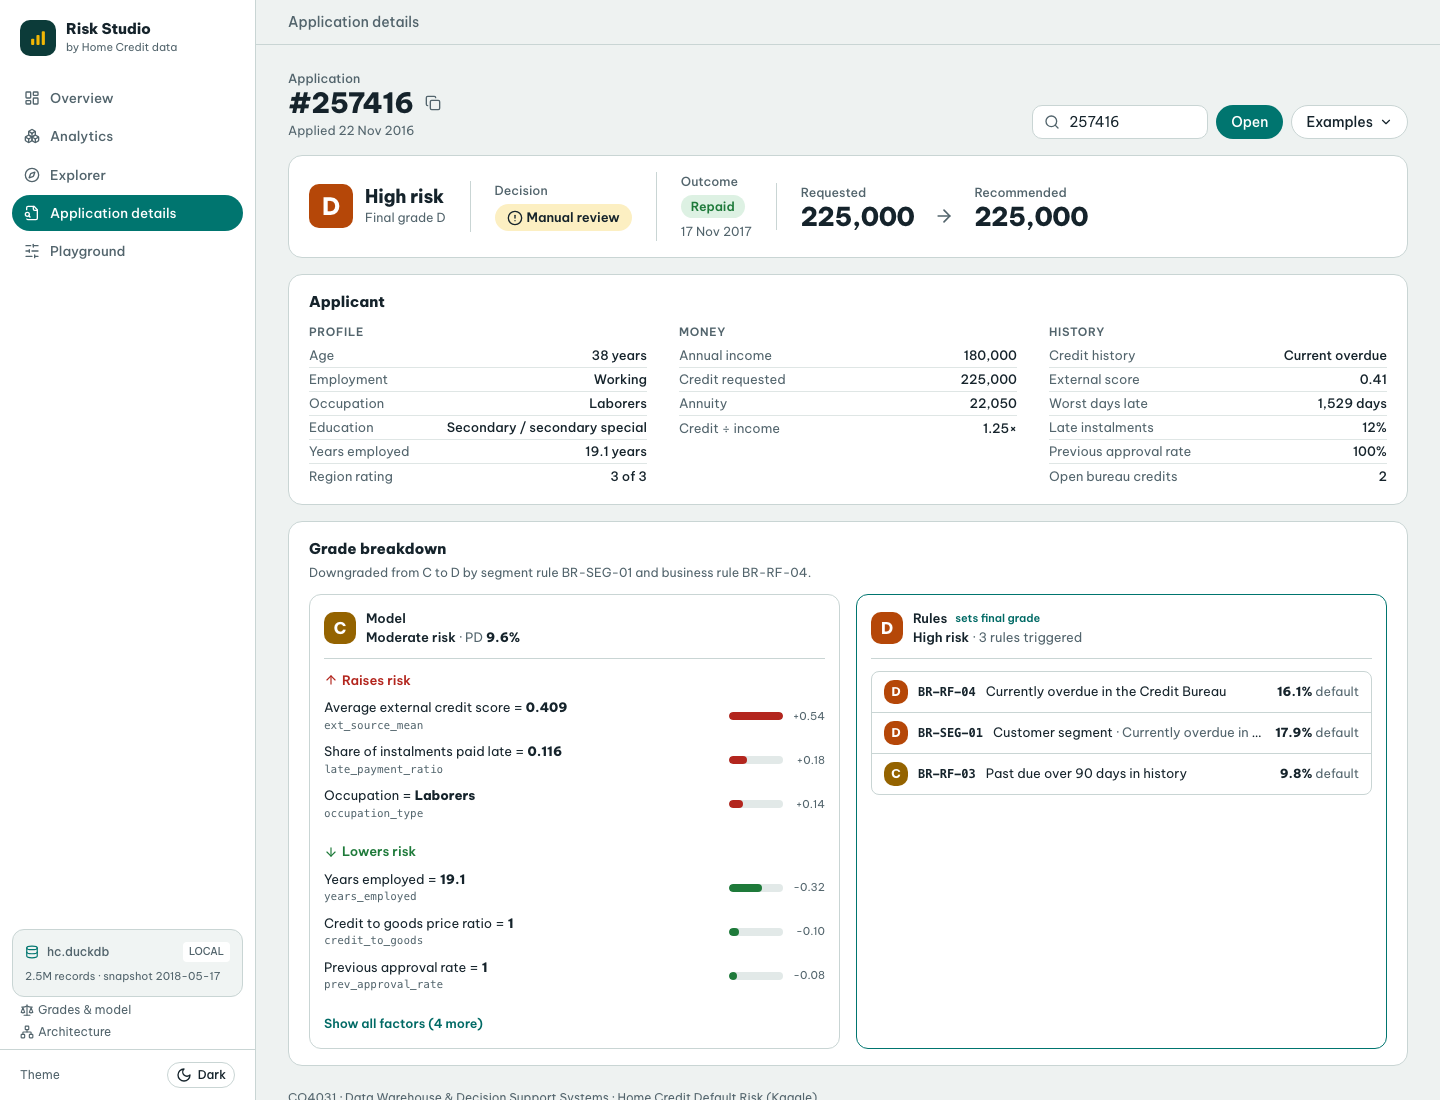
\includegraphics[width=\textwidth]{images/page_application_details.png}
	\caption{Trang chi tiết hồ sơ (\textbf{Application details})}
	\label{fig:page_application_details}
\end{figure}

\subsection{Trang Playground}
\label{sec:dss-ui-playground}

Trang \textbf{Playground} phục vụ trưởng phòng rủi ro (Q5). Hình~\ref{fig:page_playground} là trang ở chính sách hiện hành. Từ trên xuống, trang có các nút kịch bản dựng sẵn và \textbf{Reset}, năm ô KPI, \textbf{Decision mix}, bảng \textbf{Policy by grade} và thẻ \textbf{Rules}. Bảng \textbf{Policy by grade} ghi thêm số hồ sơ, tỷ lệ vỡ nợ và dư nợ chịu rủi ro của từng hạng.

\begin{figure}[H]
	\centering
	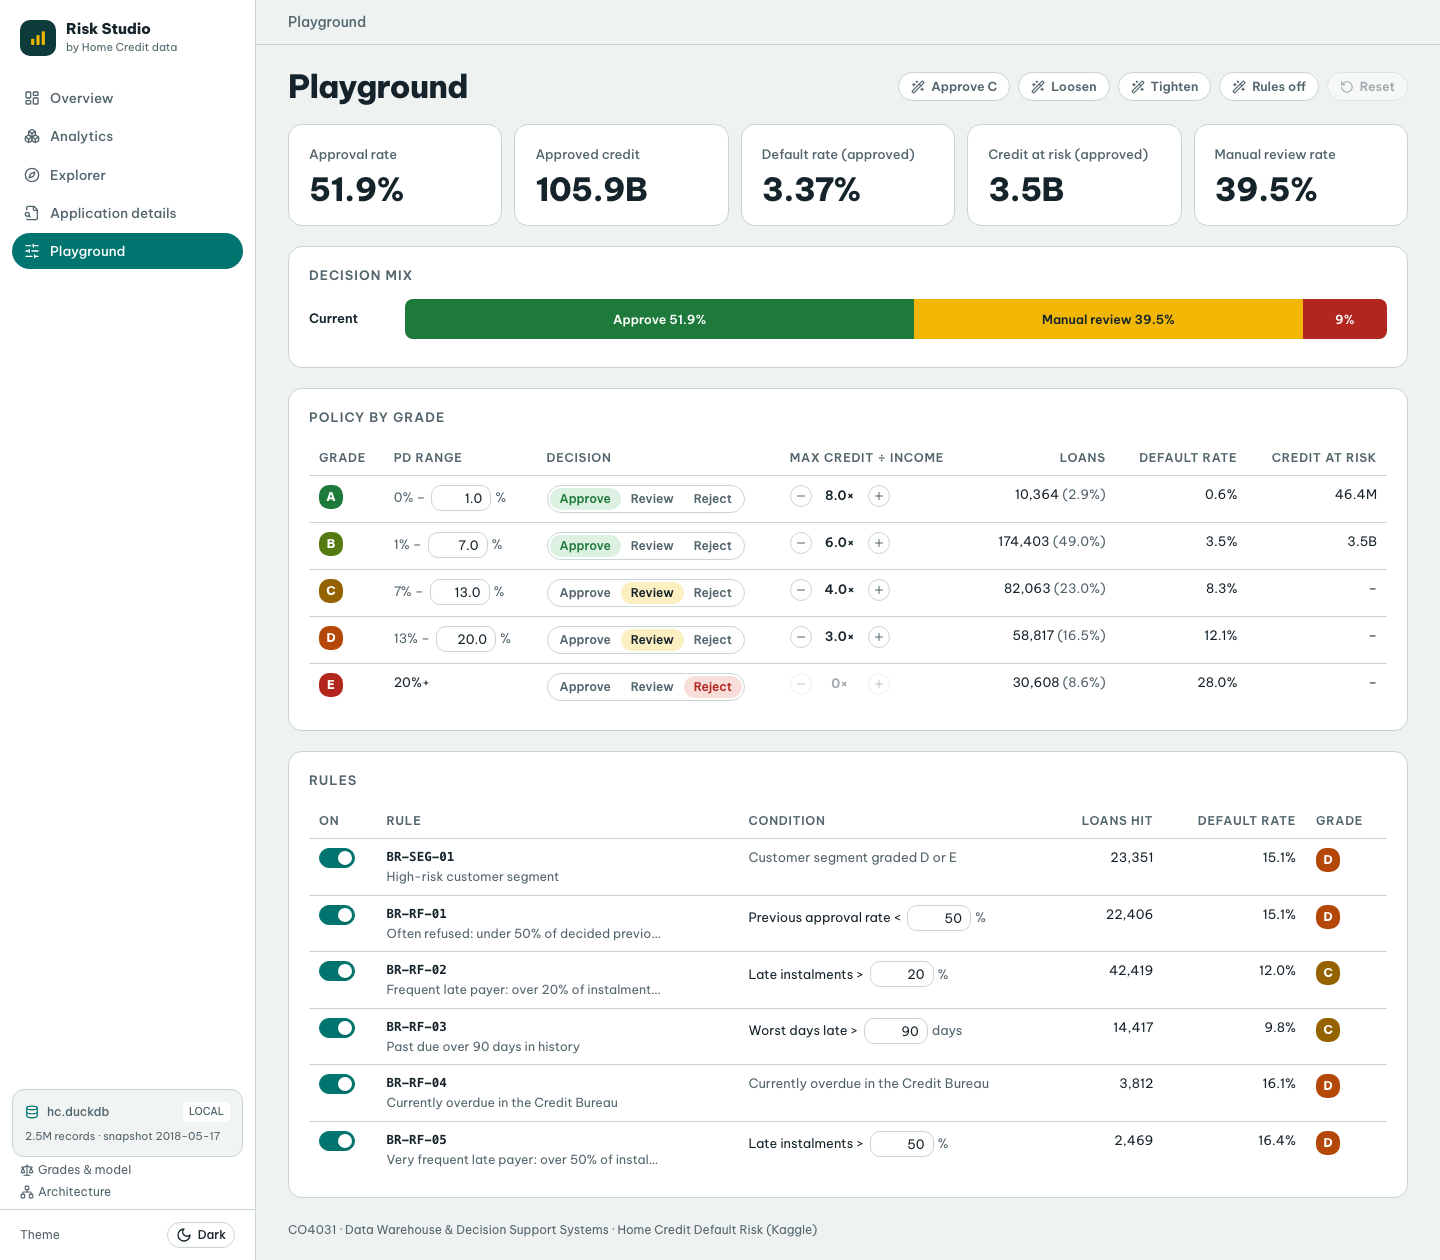
\includegraphics[width=\textwidth]{images/page_playground.png}
	\caption{Trang mô phỏng chính sách (\textbf{Playground})}
	\label{fig:page_playground}
\end{figure}

\subsection{Trang Grades \& model}
\label{sec:dss-ui-grades}

Trang \textbf{Grades \& model} là trang tham khảo về thang hạng và mô hình (BR-07, BR-11). Hình~\ref{fig:page_grades} là trang ở phạm vi \textbf{All applications}. Người dùng chọn phạm vi \textbf{All applications}, \textbf{Historical loans} hoặc \textbf{New applications}. Trang có các phần sau:
\begin{itemize}[topsep=0pt, itemsep=1pt]
	\item \textbf{Ô chỉ số:} \textbf{Downgraded by rules} ($13{,}55\%$ mọi hồ sơ) và \textbf{Model AUC} ($0{,}7586$ trên khoản vay lịch sử).
	\item \textbf{Grade scale:} Bảng hạng theo \textbf{Score}, \textbf{Rule} hoặc \textbf{Final}, với khoảng tỷ lệ, quyết định, hạn mức, tỷ trọng và tỷ lệ vỡ nợ; nhãn \textbf{Default rises A$\to$E} báo thang hạng đạt BR-07.
	\item \textbf{What drives the score:} Trung bình $|\text{SHAP}|$ của các đặc trưng, kèm nhãn \textbf{Gender not used}.
	\item \textbf{PD vs actual default:} PD trung bình so với tỷ lệ vỡ nợ thực tế theo $10$ nhóm thập phân vị PD.
\end{itemize}

\begin{figure}[H]
	\centering
	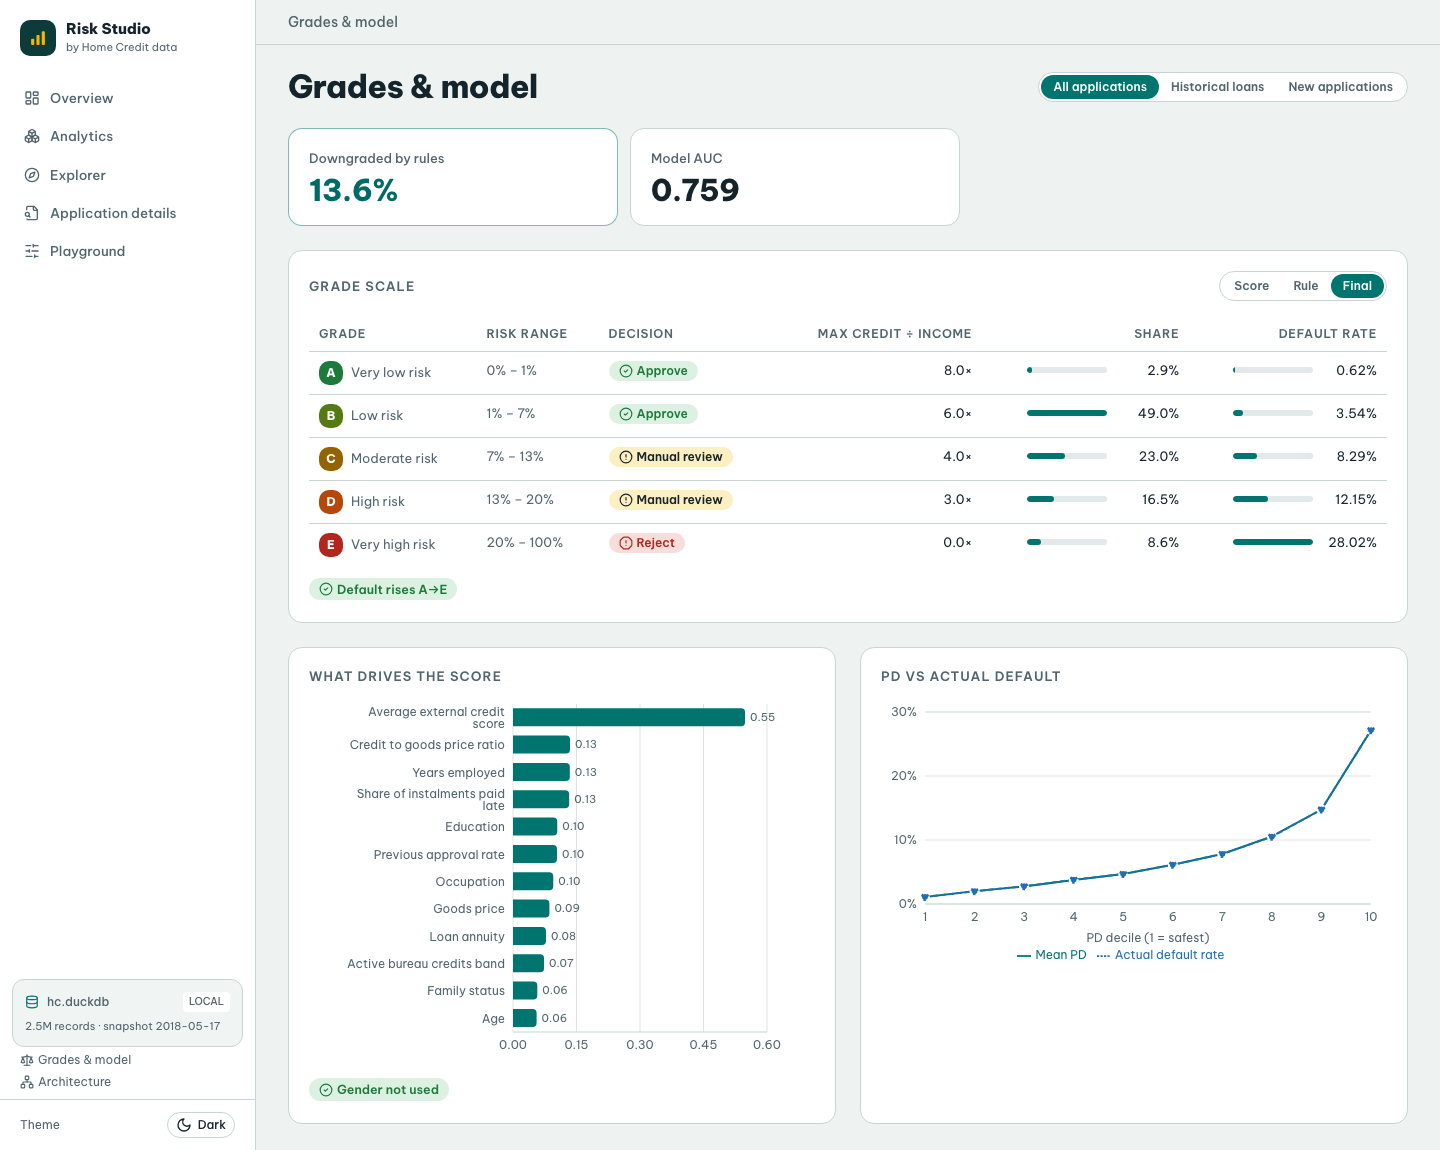
\includegraphics[width=\textwidth]{images/page_grades.png}
	\caption{Trang thang hạng và mô hình (\textbf{Grades \& model})}
	\label{fig:page_grades}
\end{figure}
\endgroup
